\documentclass{article}
\setlength{\parskip}{5pt} % esp. entre párrafos
\setlength{\parindent}{0pt} % esp. al inicio de un párrafo
\usepackage{amsmath} % mates
\usepackage{url} % que las URLs se vean lindos
\usepackage[top=25mm,left=20mm,right=20mm,bottom=25mm]{geometry} % márgenes



\usepackage[ruled,vlined]{algorithm2e}
\usepackage{algorithmic}
\usepackage{minted}
\usepackage{subcaption}
\usepackage{multicol}
\usepackage{xcolor}
\usepackage[sort&compress,numbers]{natbib} % referencias
\usepackage{minted}
\usepackage{hyperref} % ligas de URLs
\usepackage{graphicx} % poner figuras
\usepackage[spanish]{babel} % otros idiomas
\usepackage{listings}
\author{Raul L.} % author
\title{Pr\'{a}ctica 4: diagramas de Voronoi} %título
\date{\today}
\begin{document} % inicia contenido

\maketitle % cabecera


\section{Introducci\'{o}n}\label{intro} % sección y etiqueta



El tema de esta cuarta práctica tiene su importancia en las matemáticas puras y en las ciencias aplicadas como por ejemplo, en la ciencia de materiales. Se toma de un espacio bidimensional una zona con medidas conocidas que contiene $k$ puntos semillas $p_{i}$ representados por sus coordenadas $(x_{i},y_{i})$ lo que se busca es dividir esa zona en regiones llamadas celdas de Voronoi de tal forma que todos los puntos que pertenecen a la región de $p_{i}$ estén más cerca de esa semilla que de cualquier otra. \\
El modelo matemático en si es continuo, es decir, las coordenadas son números reales, pero nosotros lo vamos a discretizar en esta práctica \citep{ejemplo}.

\section{Objetivo}
Examinar el efecto de la tasa n versus k (por lo menos tres niveles de la densidad de semillas), en la probabilidad de que una segunda grieta llegue a tocar una primera grieta (es decir, fracturando la pieza dos veces con posiciones iniciales generadas independientemente al azar, sobre varias réplicas), visualizando los resultados y aplicando métodos estadísticos
\citep{ejemplo}.


\section{C\'{o}digo}
En el siguiente código se realizó un estudio cuantificando la probabilidad que hay para que dos grietas se intercepten, estas se muestran de dos diferentes colores (negro y blanco), para ello, el pixel de color rojo muestra el punto exacto de interferencia. Para realizar un concreto estudio, se varió el numero de semillas en 3 diferentes números de semillas dejando fijo el tamaño de la celda, esto garantiza realizar un estudio sistemático eficiente, el cual se representa en forma de gráfica de barras horizontales y verticales, así como también, se muestran las imágenes donde las grietas hicieron contacto con los diferentes números de semilla.

 Código en Python 

\url{https://github.com/satuelisa/Simulation/blob/master/VoronoiDiagrams/fracture.py}

**Código creado en Python**

\url{https://github.com/Raullr28/Resultados/blob/main/P4/codigo_celdas.py}
\renewcommand{\listingscaption}{Código}
\begin{listing}[H]
  \begin{minted}[linenos,mathescape,texcl]{clojure}
  
sem=8, 40, 120
porcentaje=[]
for k in sem:
    print(" semillas:",k,)
    n, semillas = 80, []
    for s in range(k):
        while True:
            x, y = randint(0, n - 1), randint(0, n - 1)
            if (x, y) not in semillas:
                semillas.append((x, y))
                break
 
    celdas = [celda(i) for i in range(n * n)]
    voronoi = Image.new('RGB', (n, n))
    vor = voronoi.load()
    c = sns.color_palette("Set3", k).as_hex()
    for i in range(n * n):
        vor[i % n, i // n] = ImageColor.getrgb(c[celdas.pop(0)])
    limite, vecinos = 10, []# se modifico para que produzca mas grietas
    for dx in range(-1, 2):
        for dy in range(-1, 2):
            if dx != 0 or dy != 0:
                vecinos.append((dx, dy))
  \end{minted}
  \label{lst:fibo}
  \caption{Representa la automatización para variar el número de semillas que aparecen.}
\end{listing}
\renewcommand{\listingscaption}{Código}
\begin{listing}[H]
  \begin{minted}[linenos,mathescape,texcl]{clojure}
 
def propaga(replica):
    prob, dificil = 0.9, 0.8
    grieta = voronoi.copy()
    g = grieta.load()
    (x, y) = inicio()
    largo = 0
    negro = (0, 0, 0)
    while True:
        g[x, y] = negro
        largo += 1
        frontera, interior = [], []
        for v in vecinos:
            (dx, dy) = v
            vx, vy = x + dx, y + dy
            if vx >= 0 and vx < n and vy >= 0 and vy < n: # existe
               if g[vx, vy] != negro: # no tiene grieta por el momento
                   if vor[vx, vy] == vor[x, y]: # misma celda
                       interior.append(v)
                   else:
                       frontera.append(v)
        elegido = None
        if len(frontera) > 0:
            elegido = choice(frontera)
            prob = 1
        elif len(interior) > 0:
            elegido = choice(interior)
            prob *= dificil
        if elegido is not None:
            (dx, dy) = elegido
            x, y = x + dx, y + dy
        else:
            break # ya no se propaga
    if largo >= limite: # aqui decide que imprima las mayores a 80 el limite
        visual = grieta.resize((10 * n,10 * n))
    return (largo, grieta)
  \end{minted}
  \label{lst:fibo}
  \caption{Representa un comando para generar la grieta.}
\end{listing}

\renewcommand{\listingscaption}{Código}
\begin{listing}[H]
  \begin{minted}[linenos,mathescape,texcl]{clojure}
 rep=400
    contacto=[]#guarda cuantas veces chocaron
    for r in range(rep): # pruebas sin paralelismo
        largo, nueva_grieta =propaga(r)# para grieta 1 color negro
        if largo > limite:
            largo2 =propaga2(r,nueva_grieta,contacto)#para grieta 2 color blanca
    print(contacto)
    probabilidad= ((len(contacto))/rep)*100#convierte a porcentaje
    porcentaje.append(probabilidad)
    print("Probabilidad de contacto entre grietas es:",probabilidad, "%")  
  \end{minted}
  \label{lst:fibo}
  \caption{Representa el lugar donde hacen contacto las grietas.}
\end{listing}

 \begin{figure}[H]
\centering
\begin{subfigure}[b]{0.35\linewidth}

\includegraphics[width=\linewidth]{imagenes/figura1.png}
\caption{Matriz 80x80}
\end{subfigure}
\begin{subfigure}[b]{0.35\linewidth}

\includegraphics[width=\linewidth]{imagenes/figura2.png}
\caption{Matriz 80x80}
\end{subfigure}
\caption{imagen de unión de grietas con igual número de semilla.}
\label{fig:westminster}
\end{figure}

\begin{figure}[H]
\centering
\begin{subfigure}[b]{0.35\linewidth}

\includegraphics[width=\linewidth]{imagenes/figura3.png}
\caption{Matriz 80x80}
\end{subfigure}
\begin{subfigure}[b]{0.35\linewidth}
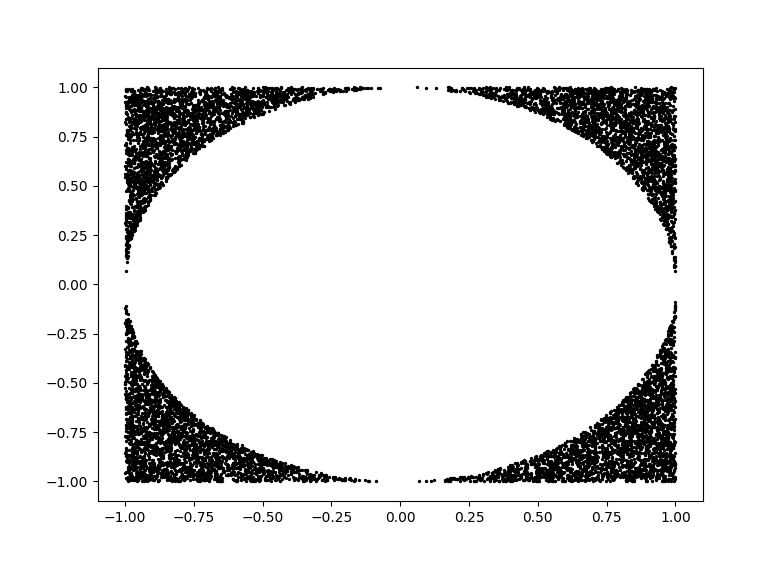
\includegraphics[width=\linewidth]{imagenes/figura4.png}
\caption{Matriz 80x80}
\end{subfigure}
\caption{imagen de unión de grietas con diferente número de semilla.}
\label{fig:westminster}
\end{figure}


 \newpage
% Computational Results
\section{Resultados}
En las figuras se muestra el porcentaje de intercepción que existió en cada uno de los diferentes números de semillas, para poder dar un resultado estadístico así, se realizó el experimento con un número alto de repeticiones lo cual nos da las gráficas siguientes.

\begin{figure}[H]
\centering
\begin{subfigure}[b]{0.50\linewidth}
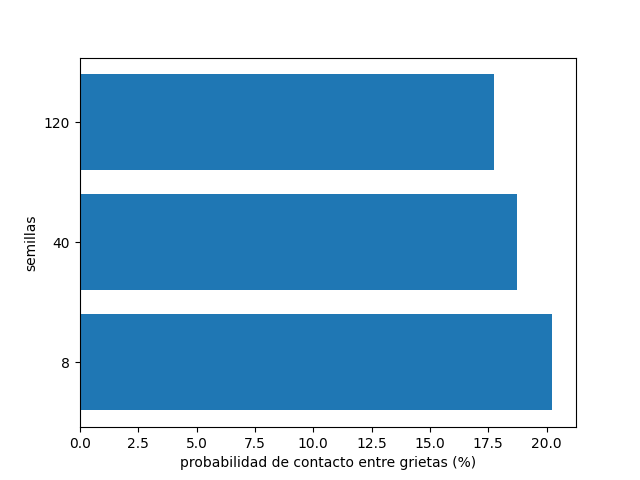
\includegraphics[width=\linewidth]{imagenes/Figure7.png}
\caption{}
\end{subfigure}
\begin{subfigure}[b]{0.50\linewidth}
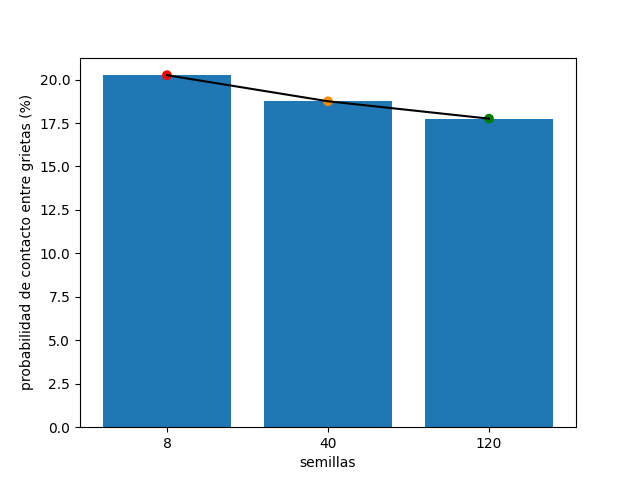
\includegraphics[width=\linewidth]{imagenes/Figure8.png}
\caption{}
\end{subfigure}
\caption{Grafica estadística de porcentaje.}
\label{fig:westminster}
\end{figure}


\newpage
\section{Reto 1}
El primer reto es crecer las celdas dinámicamente alrededor de semillas de tal forma que las semillas aparecen al azar en distintas iteraciones y crecen con una tasa exponencialmente distribuida (variable entre núcleos pero constante para un núcleo específico) hasta toparse con las demás celdas, así como se muestra en la animación. Examina los cambios producidos en el fenómeno de propagación de grietas que esta nueva forma de crear las celdas provoca, ya que las semillas resultan en celdas de tamaños distintos según su edad y su tasa, además del efecto de la posición relativa a las demas semillas.

 \begin{figure}[H]
\centering
\begin{subfigure}[b]{0.35\linewidth}

\includegraphics[width=\linewidth]{imagenes/ciclo_0.png}
\caption{ciclo 0}
\end{subfigure}
\begin{subfigure}[b]{0.35\linewidth}

\includegraphics[width=\linewidth]{imagenes/ciclo_3.png}
\caption{ciclo 3}
\end{subfigure}
\caption{Imagen de crecimiento aleatorio de semillas.}
\label{fig:westminster}
\end{figure}


 \begin{figure}[H]
\centering
\begin{subfigure}[b]{0.35\linewidth}

\includegraphics[width=\linewidth]{imagenes/ciclo_6.png}
\caption{ciclo 6}
\end{subfigure}
\begin{subfigure}[b]{0.35\linewidth}

\includegraphics[width=\linewidth]{imagenes/ciclo_9.png}
\caption{ciclo 9}
\end{subfigure}
\caption{Imagen de crecimiento aleatorio de semillas.}
\label{fig:westminster}
\end{figure}
 \begin{figure}[H]
\centering
\begin{subfigure}[b]{0.35\linewidth}

\includegraphics[width=\linewidth]{imagenes/ciclo_15.png}
\caption{ciclo 15}
\end{subfigure}
\begin{subfigure}[b]{0.35\linewidth}

\includegraphics[width=\linewidth]{imagenes/ciclo_21.png}
\caption{ciclo 21}
\end{subfigure}
\caption{Imagen de crecimiento aleatorio de semillas.}
\label{fig:westminster}
\end{figure}
\section{Resultados}
Se agregó una función donde van creciendo las semillas, cuando crece una semilla se agrega una probabilidad de que otra semilla naciera y generando un análisis de probabilidad donde se  determiná el porcentaje que aparezca otra semilla.

 \section{Conclusión}

 Se demostró que aumentando el número de repeticiones se puede tener una proporcionalidad en los resultados, demostrando así, un porcentaje alto de intercepción en las grietas con un pequeño número de semillas y por otro lado, muestra un porcentaje más pequeño con un número más pequeño de semillas.

 \bibliography{biblio.bib}
 \bibliographystyle{plainnat}

 \end{document}


